\section{Methodology}

\begin{frame}{Methodology I: Detection Architecture}
    We utilize the \textbf{YOLOv11} small architecture fine-tuned on specialized pediatric data.
    \begin{itemize}
        \item \textbf{Object Detection:} Rapid extraction of human bounding box coordinates.
        \item \textbf{Geometric Baseline:} Establishing the dimensionless Head-to-Body ratio ($R$).
    \end{itemize}
    \begin{equation}
        R = \frac{H_{total}}{H_{head}}
    \end{equation}
\end{frame}

\begin{frame}{Methodology II: Allometric Post-Processing}
    To solve the ``Invisible Child'' dyad, we evaluate spatial invariants within detected bounding boxes:
    \begin{itemize}
        \item \textbf{Vertical Displacement:} $y_{h2} < y_{h1}$ (Infers a child carried on the back).
        \item \textbf{Area Proportion:} $A_{h2} < A_{h1}$ (Confirms the secondary entity as pediatric).
    \end{itemize}
    \centering
    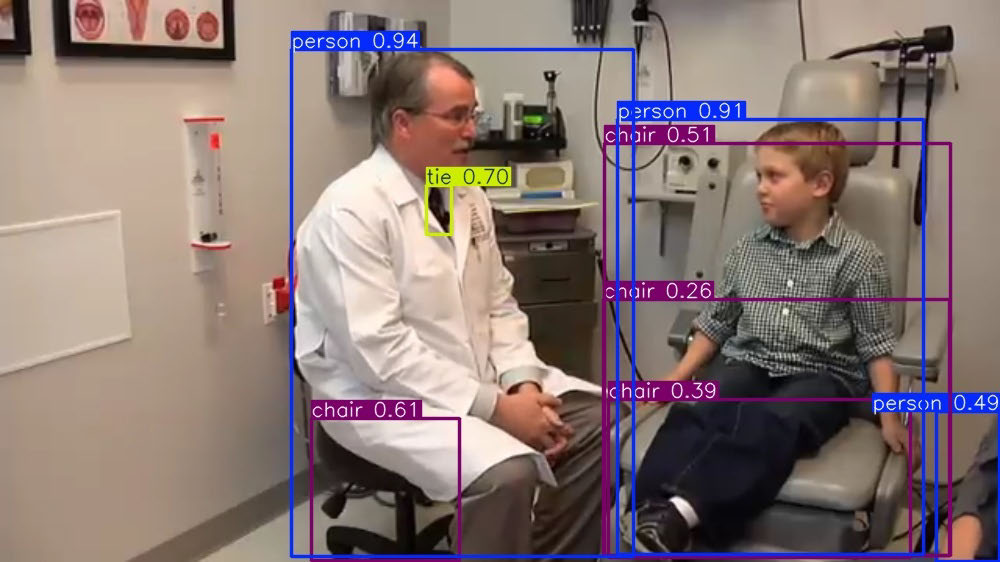
\includegraphics[width=6cm]{../research_papers/extracted_images/fig-010.jpg}
\end{frame}

\begin{frame}{Methodology III: Dataset & Verification}
    The framework is calibrated using the \textbf{Child Detection Dataset (CDD)} \parencite{diop2025}.
    \centering
    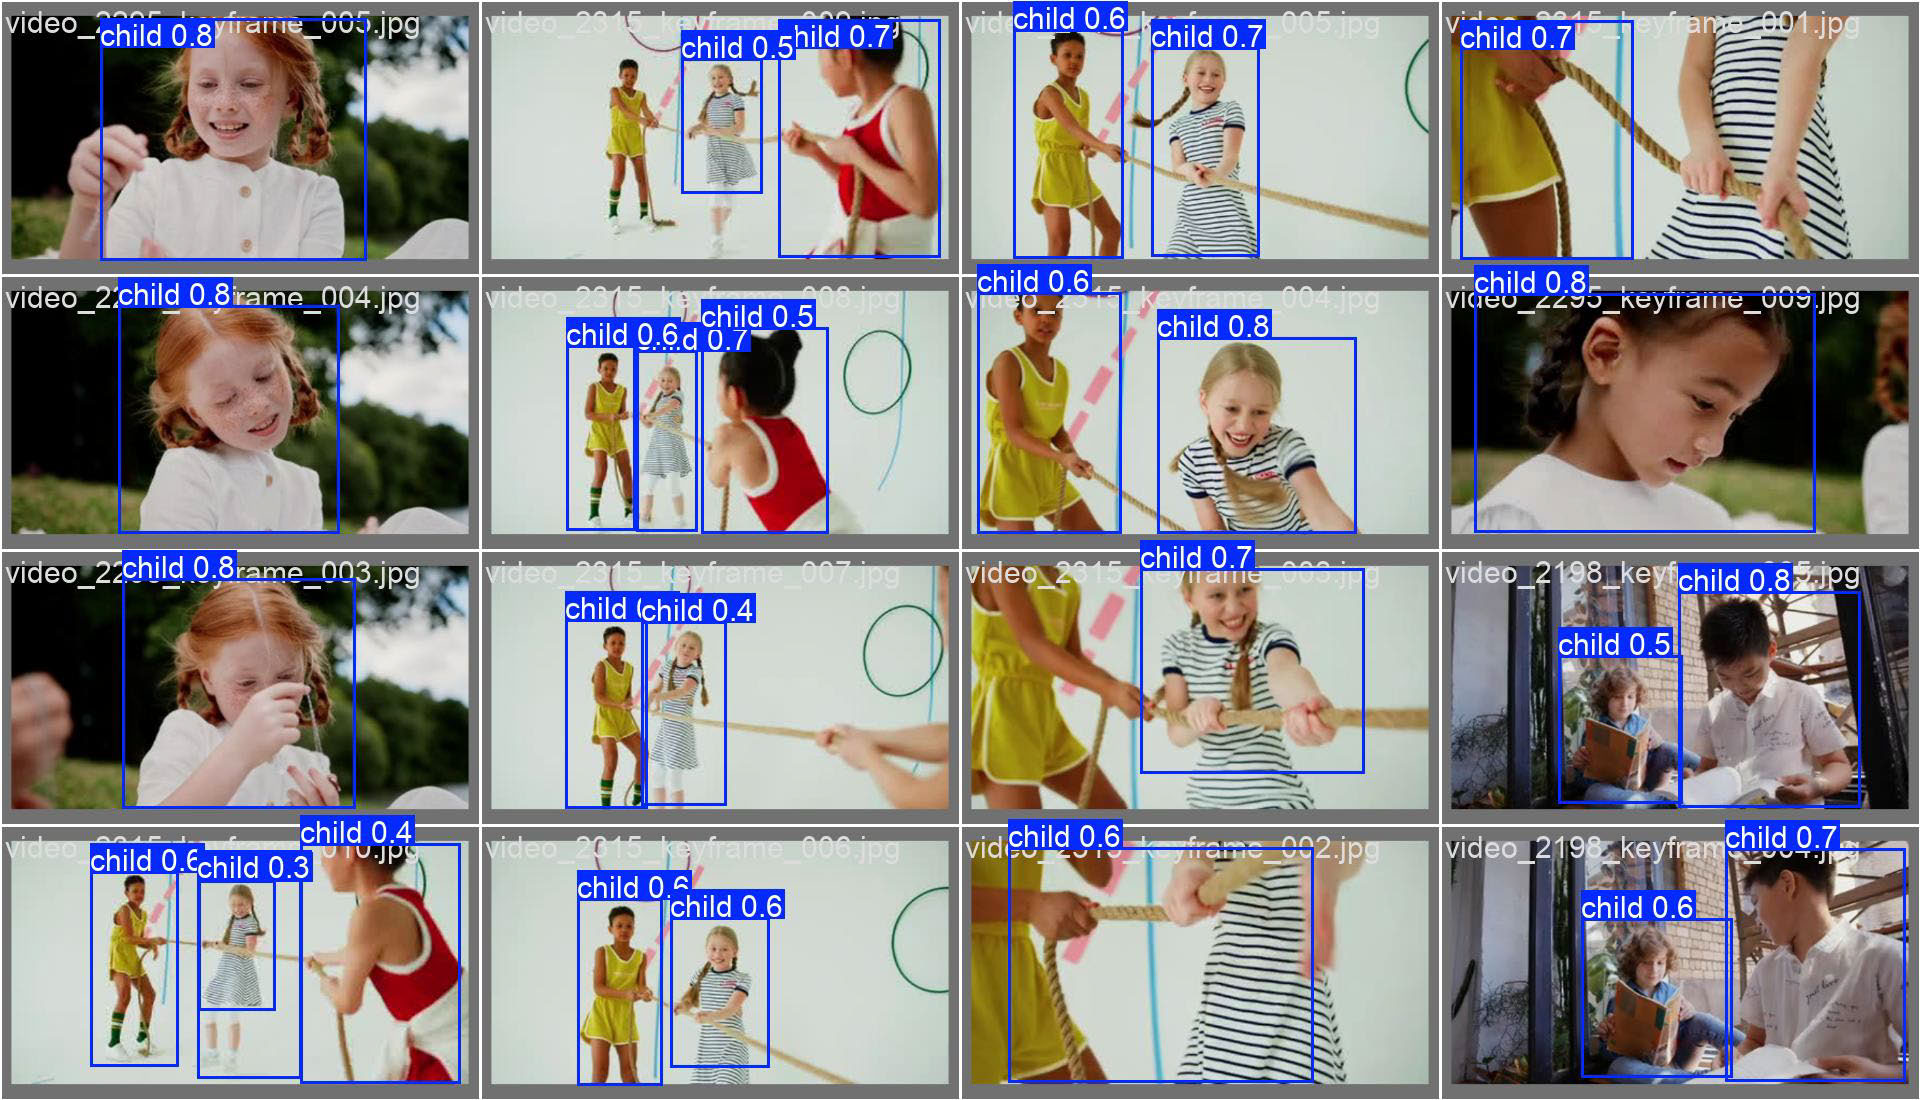
\includegraphics[width=8cm]{../research_papers/extracted_images/fig-008.jpg}
\end{frame}
